\section{Cache, Branch prediction and Translation Lookaside Buffer}

\subsection{Cache design and cache misses}
A cache is a small fast memory storage that holds the most recently used memory.
Using caches can improve the memory access time many-fold, which is important since memory access is often a bottleneck in programs.
Modern CPUs have a prefetcher that attempts to predict future memory accesses and fetches them into the cache ahead of time.
Therefore, the pattern in which a program accesses the memory can have significant influence on the performance of the program.
Modern memory systems usually have three levels of caches: Level 1 (L1), Level 2 (L2) and Level 3 (L3). \citep[Section~4.5.1]{Tanenbaum}.

\begin{figure}
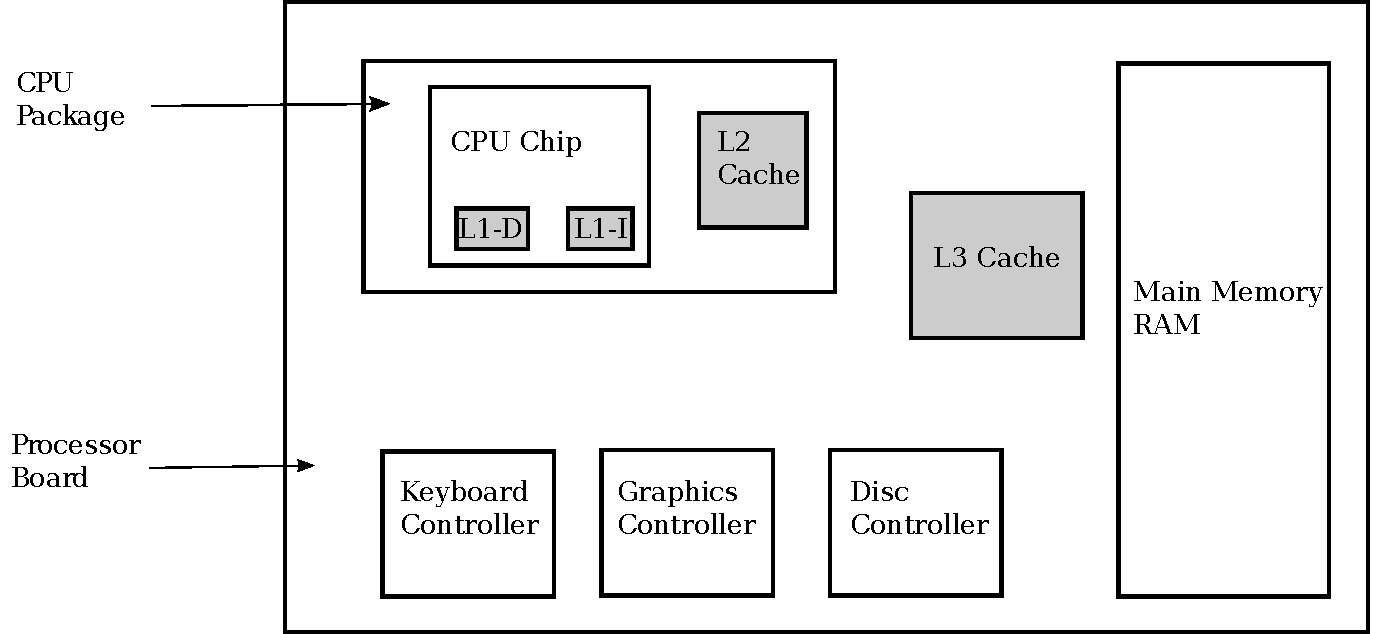
\includegraphics[width=\textwidth]{CacheLevels.pdf}
\caption{The three cache levels}
\label{fig:CacheLevels}
\end{figure}

Figure~\ref{fig:CacheLevels} \footnote{Figure borrowed from: \citep[Section~4.5.1]{Tanenbaum}} shows how the three cache are placed in the relation to the CPU. 
The L1 cache resides on the CPU chip itself and usually has a size in the range from 16 KB to 128 KB and because it is placed directly on the CPU chip it is able to provide very fast memory access.
The L2 cache is placed next to the CPU chip on the CPU package and it is connected to the CPU via a high speed path. The L2 cache typically has a size between 512 KB and 1 MB which means that it can hold more data but is not able to provide as fast access as L1.
The L3 cache is placed on the processor board and usually has a size around 3 MB. 
Since it is placed further away from the cpu it is not able to provide as fast access as L1 and L2 but still much faster than fetching data from RAM.

All three caches are inclusive which means that L2 contains the data from L1 and L3 contains the data from L2.
This means that if data is evicted from L1 it will still reside in the L2 and L3 caches or if data is evicted from L2 it will still reside in L3. 
This is an advantage because it allows fast access to data even if it is evicted from L1 or L2. 
If the caches were not inclusive then it would result in a many more data requests to the main memory.

There are two types of address locality that the caches exploit to improve performance: Spatial Locality and Temporal Locality.
Spatial Locality is that, when memory locations have addresses numerically close to a recently accessed memory location, they are more likely to be accessed soon.
Temporal Locality is that, when memory locations have been accessed recently, they are more likely to be accessed again soon.
The cache exploits spatial locality by fetching more data than has been requested, either by loading a larger chunk of memory than requested, such as a cache-line, or by speculatively fetching more cache-lines based on previously recognized access pattern.  This speculation is performed by the cache prefetcher and assumes that it is possible to anticipate future requests by looking at the previous access pattern.
Temporal locality is exploited by choosing what to evict on a cache miss and normally it is the data entries that has been accessed least recently that are evicted.

Data in the main memory is split into blocks of fixed size called \textit{cache-lines}. 
There are usually 4 to 64 consecutive bytes in a cache-line. 
Some of these cache-lines are always present in the caches. 
If a requested word is in the cache, a trip to main memory can be avoided, but if the word is not in the cache then a cache-line must be evicted from the cache (assuming that the cache is full, which it always is after the first few seconds of operation) and the cache-line containing the word must be fetched from main memory or a lower level cache if one is present. 
This is called a \textbf{cache miss} and has a high penalty because fetching a new cache-line is expensive.
The general idea is to have the most heavily used cache-lines in the caches as much of the time as possible to reduce the amount of cache misses.

\subsubsection{Cache associativity}
When designing a cache it is important to consider whether each cache-line can be stored in any cache slot or only in some of them.
There are three approaches to solving this problem; \textit{direct mapped cache}, \textit{n-way set-associative cache} and \textit{fully associative cache}. 

In a \textit{direct mapped cache} each cache-line can only be stored in a specific cache slot, the address of which is found by using a mapping function on address of the original main memory address, e.g.
\[cacheAddress = memoryAddress\bmod cacheslots\]
This means that two cache-lines cannot be mapped to the same slot simultaneously.
Given a memory address it is only necessary to look for it in one place in the cache and if it is not there then it is not in the cache. Using this approach, and an appropriate mapping function, consecutive memory lines are placed in consecutive cache slots. 
The problem with a \textit{direct mapped cache} is that since there are many more cache-lines in main memory than there are room for in the cache, many cache-lines ends up competing for the same slot. 
These competing cache-lines might end up constantly evicting each other which results in a substantial performance loss.

This problem can be fixed by using a \textit{n-way set-associative cache}, which is a cache that allows \textit{n} slots for each cache address.
This way if we have two cache-lines \textit{A} and \textit{B} whose addresses map to the same cache address and that address is already occupied by \textit{A} while \textit{B} tries to use the same address then \textit{A} does not have to be evicted because the cache has $n-1$ other slots to place \textit{B} in.
If all \textit{n} slots are occupied then a cache-line from one of them has to be evicted.
The question then becomes: Which one?

A popular algorithm, that determines which cache-lines to evict is called \textit{LRU (Least Recently Used)}.
It works by keeping an ordering of the slots at a cache address.
When a cache-line that is present in the cache is accessed the LRU algorithm updates the list by moving the entry corresponding to the accessed cache-line to the top of the list.
When an entry needs to be replaced it is the one at the end of the list that is evicted because it is the least recently used entry.

Alternatively, a \textit{fully associative cache} allows any cache-line to be saved in any cache slot but it is complicated and costly to implement in hardware because it for instance  might need to keep an ordered LRU list for the entire cache which would require a lot of bookkeeping.

The \textit{n-way set-associative cache} is the most popular choice because it has a good trade-off between implementation complexity and cache-hit rate.


\subsection{Branch Prediction and Misprediction}
There are many steps in executing a single instruction in a modern computer.
It has to be fetched, decoded, registers has to be loaded with the required data etc.
Because of this, modern computers are highly pipelined, meaning that they execute different steps for consecutive instructions in parallel.
That is, instruction 1 might be executed while instruction 2 is being decoded while instruction 3 is being fetched from the program code memory section.
A pipelined architecture can bring great speed improvement, but because of how it works, it works best on non-branching code because the result of a branch determines which instructions should be fetched, decoded and executed next.
When a branching instruction is encountered, the CPU can either choose to stall until the branching instruction has been executed, or it can try and predict the outcome of the branch before it is executed with the condition that it must be able to roll back any instructions executed between the prediction and the execution of the branching code.
Modern programs are typically full of branch instructions.

There are conditional branches and unconditional branches. 
An example of an unconditional branch and a conditional branch is shown in figure~\ref{fig:branchexample} \footnote{Example borrowed from: \citep[Section~4.5.2]{Tanenbaum}} where \textit{BNE Else} is a conditional branch and \textit{BR Next} is an unconditional branch.

\begin{figure}
\begin{algorithmic}
\If{$i = 0$}
	\State $k \gets 1$
\Else
	\State $k \gets 2$
\EndIf
\end{algorithmic}
\vspace{0.3cm}
\noindent
A possible translation to assembly looks like this:
\vspace{0.3cm}
\begin{compactenum}
\item \itab{ } \tab{\texttt{CMP} $0,1$} \tab{: compare i to 0}
\item \itab{ } \tab{\texttt{BNE Else}} \tab{: branch to \texttt{Else} if not equal}
\item \itab{\texttt{Then:}} \tab{\texttt{MOV} $k,1$} \tab{: move 1 to k}
\item \itab{ } \tab{\texttt{BR Next}} \tab{: unconditional branch to \texttt{Next}}
\item \itab{\texttt{Else:}} \tab{\texttt{MOV} $k,2$} \tab{: move 2 to k}
\item \itab{\texttt{Next:}}
\end{compactenum}
\caption{Program fragment with conditional and unconditional branches}
\label{fig:branchexample}
\end{figure}

An unconditional branch is a simple jump to a specified label, it is not based on a condition and is less of a problem than condition branches because while the target of the jump is known before the instruction is executed, it is not yet known when the fetch unit goes to fetch the next instruction.
Having no branching instructions also means the fetch unit is able to read consecutive words from memory and make better use of prefetching.

A conditional branch jumps to one of two places in the code based on whether a given condition is true of false.
The ambiguity in a conditional branch is problematic because of the nature of modern pipelined CPU architectures where the stage of the pipeline that computes the result of a comparison is many stages later than the fetching unit.
Before the result of the comparison is computed, the fetcher does not know where in the program code to fetch from.

Old pipelined machines would just stall until it was decided what branch to take. 
Doing this has a heavy impact on performance if there is a lot of conditional branches in a program, which there usually are.
Modern machines try to predict what branch is most likely to be taken, using a branch prediction unit, and then executes that code until it is known whether the branch was predicted correctly or not. 
If the branch was predicted correctly then the execution simply continues.
If the branch was mispredicted then the executed instructions in the mispredicted branch needs to be rolled back and the correct branch must be taken. 
Undoing the effects of the wrong execution path is an expensive operation which means that it is important to minimize the amount of branch mispredictions as much as possible to get good performance.

\subsubsection{Branch Prediction techniques}
There are generally two ways to do branch prediction; Static branch prediction and Dynamic branch prediction.

In \textbf{Static branch prediction} the branch taken is always fixed.
There are in general four ways to choose what branch to take and it is the compiler that chooses which to use of the first three based on where it makes sense. 
The profile-driven prediction scheme is not something that the compiler can suddenly decide to do:
\begin{description}
\item[\textbf{1. Branch always not taken:}] It is assumed that the branch is not taken which means that the instruction flow can continue as if the branch condition is false.

\item[\textbf{2. Branch always taken:}] This works in the opposite way of the above. Here it is assumed that the condition is always true and the branch is taken. This approach makes sense with a pipeline where the branch target address is known before the branch outcome.

\item[\textbf{3. Backward taken forward not taken:}] Here backward branches are always taken which for instance is the branch at the end of a loop that go back to the beginning of the next loop iteration.
The forward branches are not taken. 

\item[\textbf{4. Profile-driven prediction:}]
Here the branches of the program is profiled by running the program and the the information is given to the compiler to use for branch prediction. This of course requires the program to be compiled then run in order to be profiled and the compiled again to incorporate the branch info.
\end{description}

In \textbf{Dynamic branch prediction} the branch prediction is carried out at runtime and tries to the adapt to the program's current behaviour.
This is better than just having some static schemes to choose from because it allows more complex and usually more correct decisions.
The basic idea in dynamic branch prediction is to use the past branch behaviour to predict the future branch.

One way to do dynamic branch prediction is to have a history table that logs conditional branches as they occur, to be able to look up what direction they took when they appear again.
The simplest way to implement the history table is to have it contain one bit for each conditional branch instruction that indicates whether the conditional branch was taken or not that last time it was executed.
With this approach the branch will be predicted to go in that same direction as it did the last time. 
If the prediction is wrong the bit in the history table is flipped.

Using only one bit in the history table to indicate that a branch was take or not poses some problems.
When a loop is finished the branch at the end will always be mispredicted and change the bit in the history table.
When the loop is run again the branch at the end of the first iteration will be mispredicted.
In the case of nested loops occurring in a frequently called function, the amount of mispredictions increases and the performance suffers.

To eliminate the loop mispredictions two bits can be used in stead of one in such a way that a branch must be predicted wrong twice in a row for the prediction scheme to change.
This means that the different possible bit values becomes
00, 01, 10 and 11.
The 00 indicates that "no branch" i predicted. If this prediction is wrong the binary value gets incremented by 1 and becomes 01. Here the predicter predicts "no branch" one more time and if this is wrong the binary value is incremented again becoming 11.
If the prediction is correct then the binary value is decremented back to 00 and the prediction just continues predicting 
When the value is 11 the prediction scheme changes to "branch taken" and the prediction algorithm continues using the described approach with the only change being that the binary value is decremented in stead of incremented.

When the branch is correctly predicted there is still a problem.
The address to go to for some conditional branches are computed values obtained from doing arithmetic on registers. 
Since computation takes place after fetching, the address is unknown and the prediction becomes useless. 
A way to fix this problem is to store the address branched to last time for the particular branch, in the history table.
The previous address can then be used to branch to when the corresponding conditional branch is predicted again.


\subsection{Virtual Memory and Translation Lookaside Buffer misses}
Modern computers uses virtual memory to address the problems of sharing limited memory between processes and/or users.
Virtual memory hides the presence of physical memory and instead presents an abstract view of main memory by concealing the fact that physical memory is not allocated to a program as a single continuous region while also concealing the actual size of the main memory creating the illusion that the available memory for a given process is larger than what is physically available.
This illusion is accomplished by dividing the virtual memory into smaller subsections called \textbf{pages}, which can be loaded into physical memory when needed.
Translating a virtual address into a physical address is an expensive operation and the Translation Lookaside Buffer (TLB) helps to speed up this process.

\subsubsection{Virtual memory: Pages}
A virtual memory address \textit{va} is interpreted as a pair  containing the page number and a word number (offset within the page).
A physical memory address \textit{pa} is interpreted a pair  consisting of the page frame number and the word number within the frame, \citep[Section~8.2.1]{OperatingSystemPrinciples}.

When loading a virtual memory page into the physical memory it is  necessary to be able to translate \textit{va} to \textit{pa}.
Since the word number is the same in both \textit{va} and \textit{pa} the translation only needs to find the physical page frame that contains the virtual page.
Therefore it is necessary to keep track of the page and its current page frame which can be done using a page table.

\subsubsection{Virtual memory: Segmentation}

\begin{figure}
\center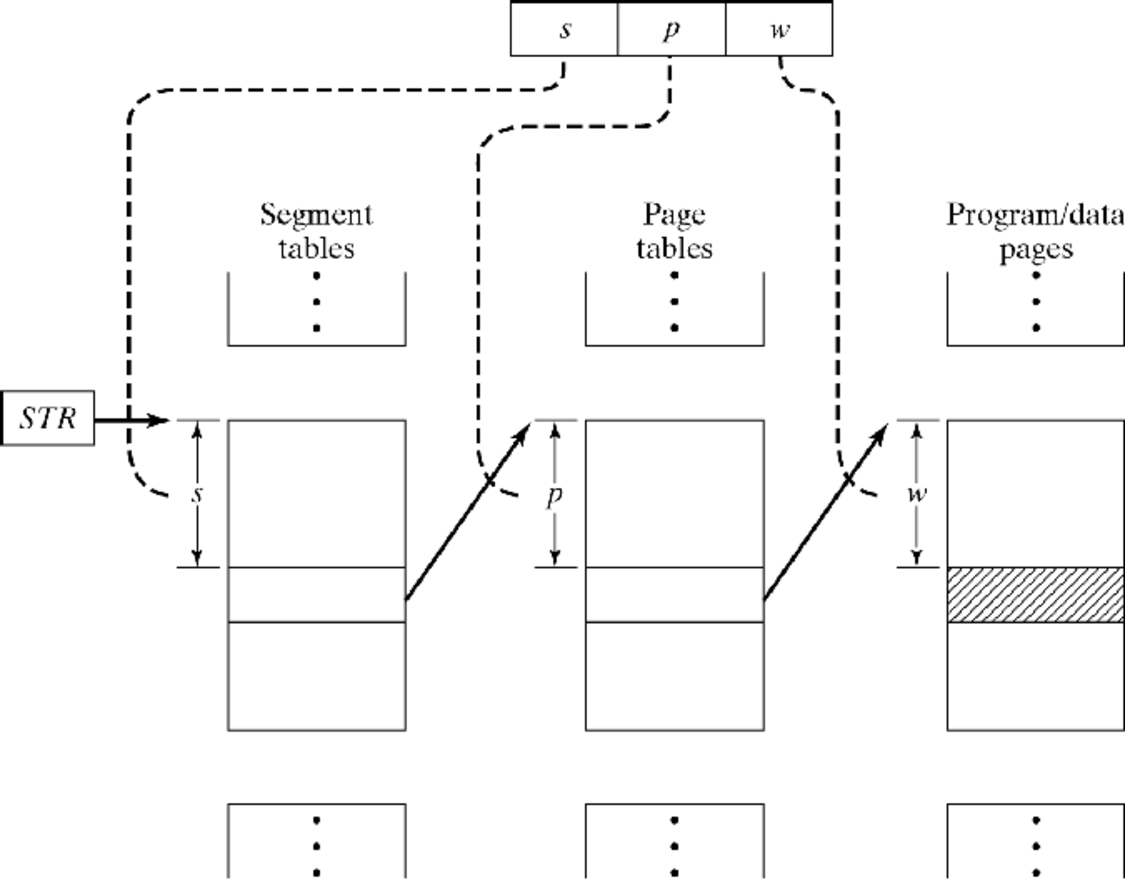
\includegraphics[width=0.70\textwidth]{virtualAddressTranslation}
\caption{Virtual Address Translation. This figure is borrowed from \citep[Figure~8-7]{OperatingSystemPrinciples}}
\label{fig:virtualAddressTranslation}
\end{figure}

Sometimes a process contains multiple dynamically changing elements. 
Placing such elements in a single address space is a difficult problem.
The problem is solved by segmentation \citep[Section~8.2.2]{OperatingSystemPrinciples}.

A segment is a collection of address spaces that can have different sizes.
This allows the virtual memory to be organized in the same way as a given application by using a segment for each logical element in the application e.g. a function, an array or table.
Segmentation and paging is combined to allow a multisegment address space while also having a simple address translation algorithm. 
The concept is shown in figure~\ref{fig:virtualAddressTranslation}.

\subsubsection{Translation Lookaside Buffer}
The translation from \textit{va} to \textit{pa} gets an extra parameter when adding segmentation; the segmentation number.
The physical address is then found by first finding the page in the segmentation table and then finding the corresponding frame in the page table and then finding the frame in the physical memory. 
This means that the translation from \textit{va} to \textit{pa} requires three physical reads.

To reduce the number of reads needed when a virtual address is translated, a translation lookaside buffer (\textbf{TLB}) is used \citep[Section~8.2.5]{OperatingSystemPrinciples}.
The TLB saves the most recent translations of \textit{va} to \textit{pa} i.e. translated pagenumbers, to make them quickly available for future use.
This means that subsequent accesses of a virtual address within a short period of time is able to bypass segmentation- and page table lookups and simply just access the needed page frame from the TLB and find it in the physical memory.
When the page is available in the TLB it is called a \textbf{TLB hit}.
The TLB is not a very large buffer though meaning that it can only hold a few virtual page translations at a time. 
A \textbf{TLB miss} occurs when a given virtual page translation is not available in the TLB and as a consequence the virtual page needs to be translated using table lookups. 
A TLB miss is therefore quite expensive and it is a good idea to minimize them as much as possible to improve performance.
